\documentclass{article}
\usepackage{amssymb, amsmath}
\usepackage{graphicx}
\usepackage{epstopdf}
\usepackage[utf8]{inputenc}
\usepackage{mdwlist}
\usepackage[left=1cm, right=2cm, top=1.5cm, bottom=1.2cm]{geometry}

\usepackage{listings}
\usepackage{color}

\definecolor{dkgreen}{rgb}{0,0.6,0}
\definecolor{gray}{rgb}{0.5,0.5,0.5}
\definecolor{mauve}{rgb}{0.58,0,0.82}

\lstset{frame=tb,
  language=Matlab,
  aboveskip=3mm,
  belowskip=3mm,
  showstringspaces=false,
  columns=flexible,
  basicstyle={\small\ttfamily},
  numbers=none,
  numberstyle=\tiny\color{gray},
  keywordstyle=\color{blue},
  commentstyle=\color{dkgreen},
  stringstyle=\color{mauve},
  breaklines=true,
  breakatwhitespace=true,
  tabsize=3
}

\epstopdfsetup{outdir=./}
\begin{document}

  \begin{enumerate*}
    \item []
    ID : 102062111, Name : Chih-Min Lin \\ \\ \\ 

    \item [1.]
    \begin{enumerate*}  
      \item [(a)] \text{}\\
      Matlab stands for "matrix" and "laboratory"
	  
      \item [(b)] \text{}\\ 
      Matlab is created by "Cleve Moler"
       
      \item [(c)] \text{}\\
      C language is used to implement the original Matlab.

      \item [(d)] \text{}\\
      LAPACK is a numerical linear algrbra package used by Matlab currently.

      \item [(e)] \text{}\\
      Yes, Matlab support symbolic computing, such as "x = 10; y = x + 100" 
    \end{enumerate*}

    \item [2.]
    \begin{enumerate*}
      \item [(a)] \text{}\\
      A Bezier curve is a mathematically defined curve used in two-dimensional graphic applications. The curve is defined by four points: the initial position and the terminating position (which are called "anchors") and two separate middle points (which are called "handles"). The shape of a Bezier curve can be altered by moving the handles.
      
      \item [(b)] \text{} \\

    \end{enumerate*}

    \item [3.]
    \begin{enumerate*}
      \item [(a)] \text{} \\
      
      \begin{lstlisting}
      x = linspace(-pi, pi);
      y = linspace(-pi, pi);
      f = sin(x) ./ x
      stem3(x, y, f)
      \end{lstlisting}
      
      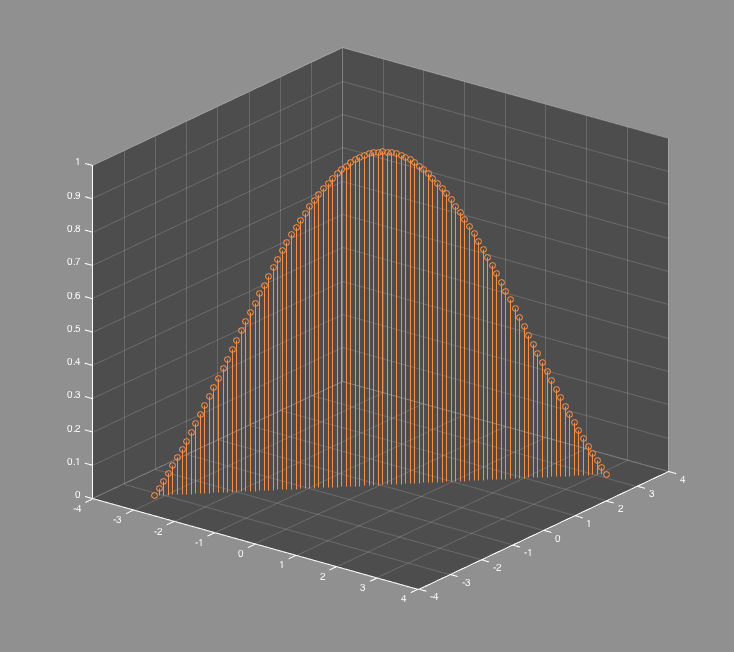
\includegraphics[width=0.7\textwidth]{/Users/chihmin/Desktop/science_computing/final/Q3_1.png}
      \ \\ 
      \ \\  
      \ \\ 
      \ \\  
    
      \item [(b)] \text{} \\
      \begin{lstlisting}
      x = linspace(-4 * pi, 4 * pi);
      y = linspace(-4 * pi, 4 * pi);
      z = abs(sin(x) ./ x);
      stem3(x, y, z)
      \end{lstlisting}
      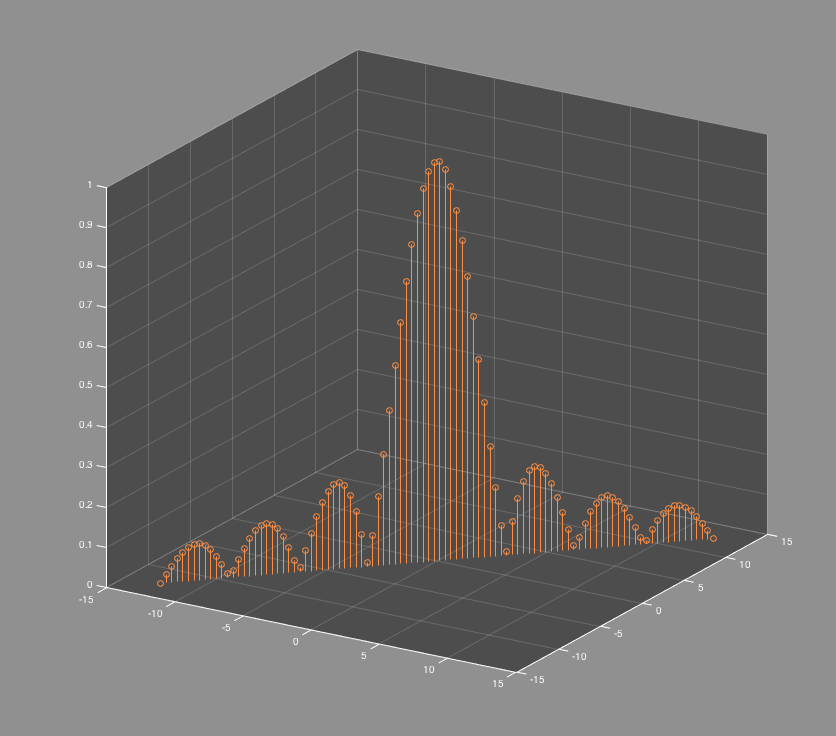
\includegraphics[width=0.7\textwidth]{/Users/chihmin/Desktop/science_computing/final/Q3_2.png}
    \end{enumerate*}
    
      \ \\ 
      \ \\  
      \ \\ 
      \ \\  
    \item [4.]
    \begin{enumerate}
      \item [(a)]
      \begin{lstlisting}
	  img = imread('58.jpg');
	  [h, w, color] = size(img)
	  B(1:color, w*h + 1) = 0;
	  for i = 1:color,
		  for j = 1:w,
			  for k = 1:h,
				  B(i, (j-1) * h + k) = img(k, j, i);
			  end
		  end
	  end

	  B(:, 1:10)  
      \end{lstlisting} \ \\ 
      Run result :
      \begin{lstlisting}
        249   245   251   245   251   255   240   248   251   245
        255   253   255   250   254   255   237   241   240   231
        255   255   255   246   247   246   222   223   218   205
      \end{lstlisting}
      
      \item [(b)]
      \begin{lstlisting}
		YUV(1, :) = 0.299 * B(1,:) + 0.587 * B(2,:) + 0.114 * B(3,:);
		YUV(2, :) = -0.147 * B(1,:) - 0.289 * B(2,:) + 0.436 * B(3,:);
		YUV(3, :) = 0.615 * B(1,:) - 0.515 * B(2,:) - 0.1 * B(3,:);

		for j = 1:w,
			for k = 1:h,  
				Y(k, j) = B(1, (j-1) * h + k);
				U(k, j) = B(2, (j-1) * h + k);
				V(k, j) = B(3, (j-1) * h + k);
			end
		end
		imshow([Y, U, V]);
      \end{lstlisting} \ \\
	  Origin picture : \ \\ \ \\ 
      
\includegraphics[width=0.7\textwidth]{/Users/chihmin/Desktop/science_computing/final/58.jpg} \ \\
      Output picture : \ \\ \ \\
      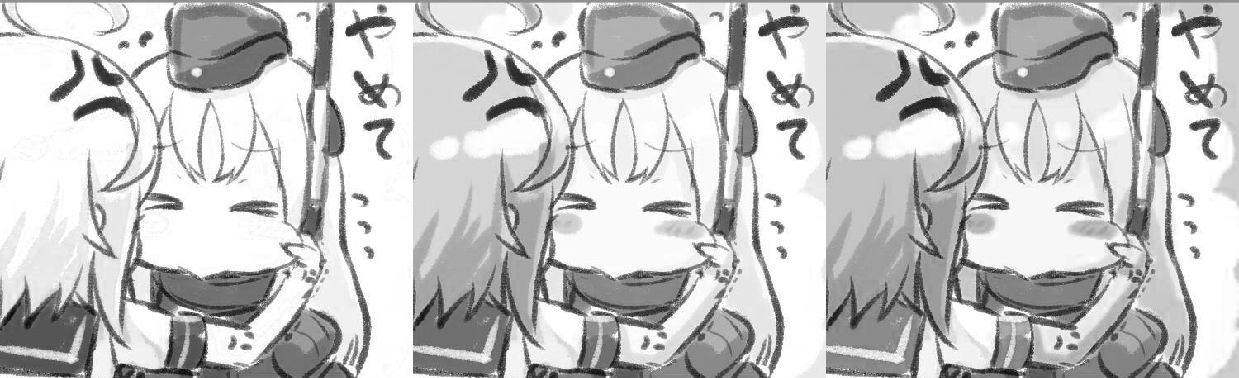
\includegraphics[width=0.7\textwidth]{/Users/chihmin/Desktop/science_computing/final/Q4_b.png}
	
    \end{enumerate} \ \\ \ \\  
    
    \item [6.] 
     \begin{enumerate}
       \item [(a)] \text{}
          \begin{align*}
            \text{we knows that :} & \frac{x^2}{a^2} + \frac{y^2}{b^2}  = 1  \\
            Y & = y^2 = \alpha X + \beta = - \frac{b^2}{a^2} x^2 + b^2 \\
            a^2 & = -\frac{\beta}{\alpha},\ b^2 = \beta \\
            Original\ equation\ is & \ (x-a)^2+(y-b)^2=c^2\ is\ also\ equal\ to\  \frac{(x-a)^2}{c^2} + \frac{(y-b)^2}{c^2}=1 \\ 
            \because &\text{We don't care about the offset of x and y corrdinate}\\
            \therefore& \ The\ linear\ equation\ is\ y^2=-\frac{c^2}{c^2}x^2+c^2,\ Y=-X+c^2
          \end{align*}
        
        \item [(b)] \text{}
          \begin{align*}
            \text{We know the linear equation of } & y=\frac{ax}{x^2+b^2}\ is \\
            & \frac{1}{y} = \frac{1}{a}x+\frac{b^2}{a}\frac{1}{x} \\
            & Let\  Y=\frac{1}{y},\ \alpha=\frac{1}{a},\ \beta=\frac{b^2}{a} \\
            & \therefore Y = \alpha x+\beta\frac{1}{x}
          \end{align*}

        \item [(c)] \text{}
          \begin{align*}
            \text{We know the linear equation of } & \frac{x^2}{a^2}+\frac{y^2}{b^2}=1\ is \\
            & y^2 = -\frac{b^2}{a^2}x^2+b^2\\
            & Let\  Y=y^2,\ \alpha=-\frac{b^2}{a^2},\ \beta=b^2 \\
            & \therefore Y = \alpha x^2+\beta
          \end{align*}
     \end{enumerate}
     \item [7.]
      \begin{enumerate}
        \item [(a)] \text{} \\
        \begin{lstlisting}
        Fs=16000;
        Ts=1/Fs;
        t=[0:Ts:4];
        [~, length] = size(t);

        music = t;
        step = length / 800; 
        for i = 1:length,
            hz = i / step;
          music(i) = sin(2 * pi * hz * t(i));
        end

        plot(t, music)
        \end{lstlisting} \ \\
        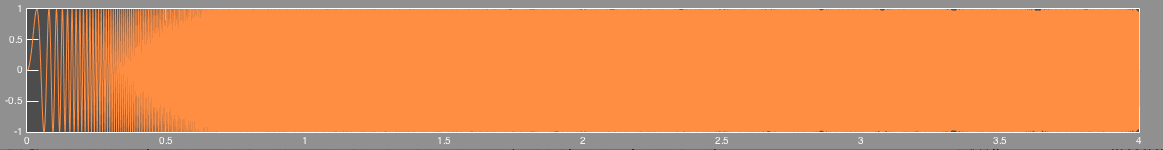
\includegraphics[width=0.9\textwidth]{/Users/chihmin/Desktop/science_computing/final/sound.png}

        \item [(b)] \text{} \\
        \begin{lstlisting}
          plot(t(1:10000), music(1:10000)); 
        \end{lstlisting} 
        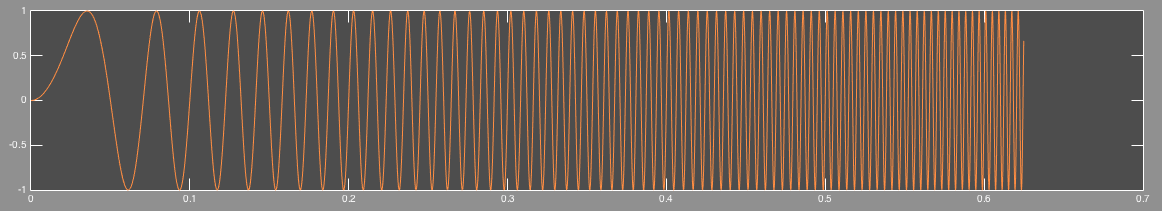
\includegraphics[width=0.9\textwidth]{/Users/chihmin/Desktop/science_computing/final/sound2.png}
        
        \item [(c)] \text{} \\
        I think this is the same because we just up-side-down the value of y, and y is a sin function.
      \end{enumerate}
        
  \end{enumerate*}
\end{document}

